\documentclass[border=5mm]{standalone}
\usepackage{pgfplots}
\usetikzlibrary{arrows.meta}
\pgfplotsset{compat=1.18}

\begin{document}
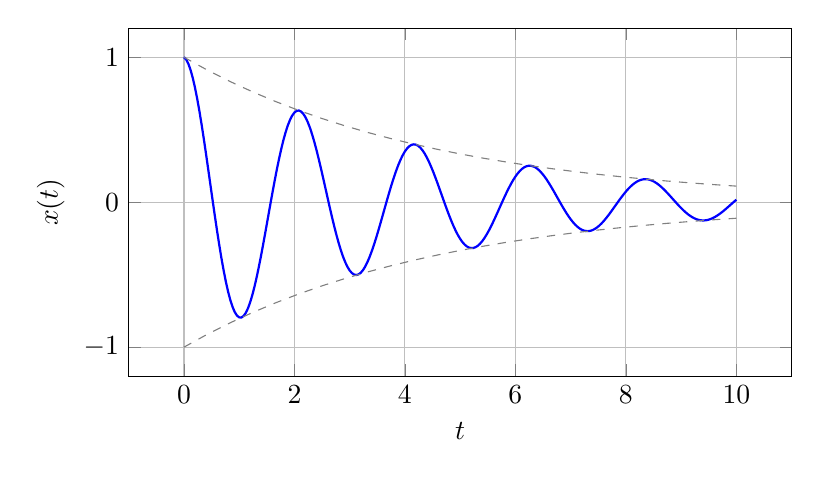
\begin{tikzpicture}[>=Stealth]
\begin{axis}[width=10cm,height=6cm,grid=major,xlabel={$t$},ylabel={$x(t)$}]

\addplot[blue,thick,domain=0:10,samples=251]{exp(-.22*x)*cos(deg(3*x))};
\addplot[gray,dashed,domain=0:10]{exp(-.22*x)};\addplot[gray,dashed,domain=0:10]{-exp(-.22*x)};
\end{axis}
\end{tikzpicture}
\end{document}
